\begin{figure}
    \centering
    %Chart: Mean scores (Dimension 5)
    \begin{tikzpicture}
        \begin{axis}[
            axis lines=left,
            axis x line=bottom,
            axis line style={draw=black,-},
            width  = .85\textwidth,
            height = .25\textheight,
            major x tick style = transparent,
            ybar=3.0*\pgflinewidth,
            bar width=6pt,
            xmajorgrids = true,
            ymajorgrids = false,
            yticklabels={},
            ylabel = {\scriptsize Mean score},
            symbolic x coords={Academic prose,Official documents,Religion,Hobbies,Press reviews,Press reportage,Professional letters,Press editorials,Popular lore,Humor,Biographies,Broadcasts,Prepared speeches,Interviews,Adventure fiction,General fiction,Science fiction,Spontaneous speeches,Mystery fiction,Personal letters,Romantic fiction,Face-to-face conversations,Telephone conversations},
            xtick = data,
            nodes near coords,
            every node near coord/.append style={/pgf/number format/fixed},
            every node near coord/.append style={font=\tiny},
            every node near coord/.append style={rotate=90,anchor=west},
            nodes near coords style={/pgf/number format/.cd,precision=1},
            every axis/.append style={label style={font=\footnotesize},tick label style={font=\footnotesize}},
            x tick label style={rotate=30,anchor=east,font=\tiny,xshift=5pt},
            scaled y ticks = false,
            enlarge y limits={abs=.2*\pgfplotbarwidth},
            enlarge x limits={abs=1.5*\pgfplotbarwidth},
            extra y ticks = 0,
            extra y tick labels={},
            extra y tick style={grid=major,major grid style={thick,densely dashed,draw=red}}
        ]
        \addplot[style={draw=black,fill=red!50,mark=none}]
            coordinates {
                (Academic prose,5.5)
                (Official documents,4.7)
                (Religion,1.4)
                (Hobbies,1.2)
                (Press reviews,0.8)
                (Press reportage,0.6)
                (Professional letters,0.4)
                (Press editorials,0.3)
                (Popular lore,0.1)
                (Humor,-0.4)
                (Biographies,-0.5)
                (Broadcasts,-1.7)
                (Prepared speeches,-1.9)
                (Interviews,-2.0)
                (Adventure fiction,-2.5)
                (General fiction,-2.5)
                (Science fiction,-2.5)
                (Spontaneous speeches,-2.6)
                (Mystery fiction,-2.8)
                (Personal letters,-2.8)
                (Romantic fiction,-3.1)
                (Face-to-face conversations,-3.2)
                (Telephone conversations,-3.7)
            };
        \end{axis}
    \end{tikzpicture}
    \hspace*{4pt}
    %Chart: Loadings (Dimension 5)
    \begin{tikzpicture}
        \begin{axis}[
            axis lines=left,
            axis x line=bottom,
            axis line style={draw=black,-},
            width  = .85\textwidth,
            height = .25\textheight,
            major x tick style = transparent,
            ybar=3.0*\pgflinewidth,
            bar width=6pt,
            xmajorgrids = true,
            ymajorgrids = false,
            yticklabels={},
            ylabel = {\scriptsize Loading},
            symbolic x coords={Conjuncts,Agentless passives,Past participal clauses,BY-passives,Past participial WHIZ deletions,Other adverbial subordinators,Predicative adjectives,Type-token ratio},
            xtick = data,
            nodes near coords,
            every node near coord/.append style={/pgf/number format/fixed},
            every node near coord/.append style={font=\tiny},
            every node near coord/.append style={rotate=90,anchor=west},
            nodes near coords style={/pgf/number format/.cd,precision=1},
            every axis/.append style={label style={font=\footnotesize},tick label style={font=\footnotesize}},
            x tick label style={rotate=45,anchor=east,font=\tiny,xshift=5pt},
            scaled y ticks = false,
            enlarge y limits={abs=.2*\pgfplotbarwidth},
            enlarge x limits={abs=1.5*\pgfplotbarwidth},
            extra y ticks = 0,
            extra y tick labels={},
            extra y tick style={grid=major,major grid style={thick,densely dashed,draw=red}}
        ]
        \addplot[style={draw=black,fill=blue!25,mark=none}]
            coordinates {
                (Conjuncts,0.48)
                (Agentless passives,0.43)
                (Past participal clauses,0.42)
                (BY-passives,0.41)
                (Past participial WHIZ deletions,0.40)
                (Other adverbial subordinators,0.39)
                (Predicative adjectives,0.31)
                (Type-token ratio,-0.31)
            };
        \end{axis}
    \end{tikzpicture}
    \caption{Dimension 5 -- Abstract versus Non-Abstract Style \citep{biberVariationSpeechWriting1988}}
    \label{fig:merged_dim5_biber}
\end{figure}
